\begin{minipage}{\textwidth}
	\begin{minipage}{0.6\textwidth}
		
		\item Una barra uniforme de masa $m$ y largo $L$ se encuentra unida en su extremo a un resorte de constante elástica $k$. Esta barra está pivoteada a $3L/10$ de uno de sus extremos como se muestra en la figura. Considere que la barra se desplaza un ángulo pequeño $\theta$ con respecto a la vertical. Recuerde que el momento de inercia de una barra de largo $L$ y masa $M$ respecto al centro de masa es $\frac{1}{12}ML^2$.
		\begin{enumerate}[a)]
			\item Determine la ecuación de movimiento del sistema y su frecuencia natural.
			\item Si el sistema se ve sometido a una fuerza armónica externa $F(t)=F_0 \cos(\Omega t)$ y a una fuerza de roce proporcional a la velocidad del centro de masa, con una constante de proporcionalidad $b$, ambas fuerzas aplicadas en el centro de masa de la barra. Determine la frecuencia de resonancia $\Omega_R$.
			\item Determine la potencia disipada debida a la fuerza de roce del estado estacionario y la potencia promedio $\bar{P}$ en un período de tiempo.
		\end{enumerate}
		
		\begin{equation*}
		\bar{P} = \dfrac{1}{T} \int_0^TP(t)dt
		\end{equation*}
		
	\end{minipage}
	\begin{minipage}{0.4\textwidth}
		
		\vspace{-3cm}
		\begin{center}
			\begin{tikzpicture} [rotate=20,scale=.7]
			%control1a%
			\filldraw [fill=white!50!gray] (0,0) rectangle (1,-10);
			\fill [fill=white] (.5,-3) circle (.2);
			\begin{scope}[shift={(0,-10)},rotate=-20]
			\draw [thick, decoration={aspect=0.4, segment length=3.5mm, amplitude=4mm, coil}, decorate] (-.5,0)--(-4.5,0);
			\draw [thick] (-7,10)--(-5,10)--(-5,-2)--(-7,-2) (0,0)--(-.5,0) (-4.5,0)--(-5,0);
			\fill [pattern = north west lines] (-7,10) rectangle (-5,-2);
			\end{scope}
			\begin{scope}[shift={(.5,-3)}]
			\draw [thick,rotate=-20,dashed] (0,0)--(0,-6); 
			\end{scope}
			\draw [thick] (0,0)--(-.4,0) (0,-3)--(-.4,-3) (-.2,0)--(-.2,-3);
			\draw [white,thick,dashed] (0.5,-3)--(0.5,-9.9);
			\draw [thick,dashed] (-1.25,-8) arc (245:285:2.6);
			\draw [dotted]
			(-1,-2) node[scale=1] {\(\frac{3}{10}L\)}
			(-3,-8) node[scale=1] {K}
			(-.3,-7) node[scale=1] {\(\theta\)}
			(2,-9) node[scale=1] {\(L,m\)}
			;
			\end{tikzpicture}
		\end{center}
		
	\end{minipage}
\end{minipage}

\textbf{\underline{Solución:}}

\begin{enumerate}[a)]

\item \textbf{DCL}
\begin{minipage}{0.3\textwidth}
	\begin{figure}[H]
		\centering
		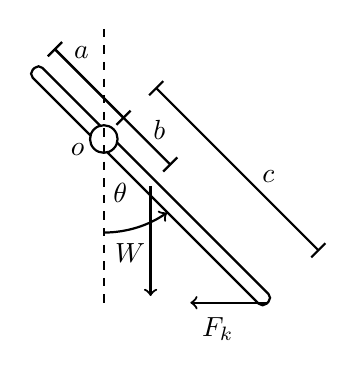
\begin{tikzpicture}[scale=1.4,rotate=-45]
		\draw [thick,rounded corners=2pt] (0,2)rectangle(3,1.875);
		\draw [thick,|-|] (0,2.2)--(.9,2.2); 
		\draw [thick,|-|] (0,2.2)--(1.5,2.2);
		\draw [thick,|-|] (.9,2.6)--(3,2.6);
		\filldraw [thick,fill=white] (.9,1.9375)circle(.125);
		\begin{scope}[shift={(1.5,1.9375)}]
		\draw [thick,->,rotate=-45] (0,0)--(1,0);
		\end{scope}
		\begin{scope}[shift={(.9,1.9375)}]
		\draw [thick, dashed, rotate=-45] (-1,0)--(1.5,0);
		\draw [thick, ->] (.6,-.6)arc(315:350:1);
		\end{scope}
		\begin{scope}[shift={(3,1.9375)}]
		\draw [thick, ->, rotate=-135] (0,0)--(.7,0);
		\end{scope}
		\draw [dotted]
			(.2,2.35) node {\(a\)}
			(1.2,2.35) node {\(b\)}
			(2.2,2.75) node {\(c\)}
			(.8,1.7) node {\(o\)}
			(1.35,1.7) node {\(\theta\)}
			(1.8,1.375) node {\(W\)}
			(2.85,1.45) node {\(F_k\)}
			;
		\end{tikzpicture}
	\end{figure}
\end{minipage}
\hspace{0.05\textwidth}
\begin{minipage}{0.55\textwidth}
\begin{align*}
a=\frac{3L}{10} \, , \, d=\frac{L}{5} \, ,\, c=\frac{7L}{10}\\
\circlearrowleft\Sigma\tau_0=-Wd\sin\theta -F_kc\cos\theta=I_0\ddot\theta
\end{align*}
donde \(W=mg\), \(F_k=kc\sin\theta\), suponiendo que \(\theta\) mide desde la posición de equilibrio.
\end{minipage}



Por otro lado:
\begin{equation*}
I_0=I_{cm}+md^2=\frac{1}{12}mL^2+m\frac{L^2}{25}=\frac{37}{300}mL^2
\end{equation*}
entonces, con \(\theta\approx\sin\theta\) para \(\theta\approx0\)
\begin{align*}
-mgd\theta-Kc^2\theta=I_0\ddot\theta&\Rightarrow\ddot\theta+\left(\frac{mgd}{I_0}+\frac{Kc^2}{I_0}\right)\theta\\
\end{align*}
\begin{equation*}
\tcbhighmath{\Rightarrow\ddot\theta+\left(\frac{60}{37}\cdot\frac{g}{L}+\frac{147}{37}\cdot\frac{K}{m}\right)\theta=0}
\end{equation*}
\begin{equation*}
\tcbhighmath{\wedge  \omega_n=\sqrt{\frac{60}{37}\cdot\frac{g}{L}+\frac{147}{37}\cdot\frac{K}{m}}}
\end{equation*}

\item \textbf{DCL}

\begin{minipage}{0.3\textwidth}
	\begin{figure}[H]
		\centering
		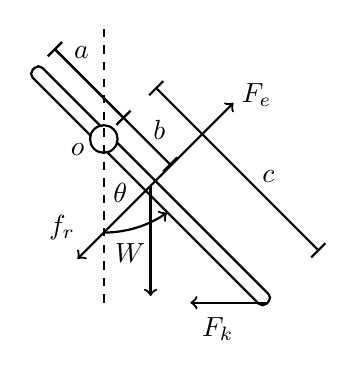
\begin{tikzpicture}[scale=1.4,rotate=-45]
		\draw [thick,rounded corners=2pt] (0,2)rectangle(3,1.875);
		\draw [thick,|-|] (0,2.2)--(.9,2.2); 
		\draw [thick,|-|] (0,2.2)--(1.5,2.2);
		\draw [thick,|-|] (.9,2.6)--(3,2.6);
		\draw [thick, <->] (1.5,1)--(1.5,3);
		\filldraw [thick,fill=white] (.9,1.9375)circle(.125);
		\begin{scope}[shift={(1.5,1.9375)}]
		\draw [thick,->,rotate=-45] (0,0)--(1,0);
		\end{scope}
		\begin{scope}[shift={(.9,1.9375)}]
		\draw [thick, dashed, rotate=-45] (-1,0)--(1.5,0);
		\draw [thick, ->] (.6,-.6)arc(315:350:1);
		\end{scope}
		\begin{scope}[shift={(3,1.9375)}]
		\draw [thick, ->, rotate=-135] (0,0)--(.7,0);
		\end{scope}
		\draw [dotted]
		(.2,2.35) node {\(a\)}
		(1.2,2.35) node {\(b\)}
		(2.2,2.75) node {\(c\)}
		(.8,1.7) node {\(o\)}
		(1.35,1.7) node {\(\theta\)}
		(1.8,1.375) node {\(W\)}
		(2.85,1.45) node {\(F_k\)}
		(1.6,3.2) node {\(F_e\)}
		(1.2,1.1) node {\(f_r\)}
		;
		\end{tikzpicture}
	\end{figure}
\end{minipage}
\hspace{0.05\textwidth}
\begin{minipage}{0.55\textwidth}
\begin{equation*}
\circlearrowleft\Sigma\tau_0=-Wd\sin\theta-F_xc\cos\theta-f_rd+F_ed=I_0\ddot\theta
\end{equation*}
con \(f_r=bd\dot\theta\wedge F_e=F_0\cos(\Omega t)\)
\begin{equation*}
\Rightarrow \ddot\theta+\frac{bd^2}{I_0}\dot\theta+\left(\frac{mgd}{I_0}+\frac{Kc^2}{I_0}\right)\theta=\frac{F_0d}{I_0}\cos(\Omega t)
\end{equation*}
\end{minipage}

De la ecuación de movimiento se desprende: \(\gamma=\frac{bd^2}{2I_0}\), además la amplitud estacionaria del movimiento es:
\begin{align*}
&Ae=\frac{\frac{F_0d}{I_0}}{\sqrt{{\left({\omega_n}^2-\Omega^2\right)}^2-4\gamma^2\Omega^2}}=\frac{F_0d}{I_0}{\left[{\left({\omega_n}^2-\Omega^2\right)}^2-4\gamma^2\Omega^2\right]}^{-\frac{1}{2}}\\
\Rightarrow &\frac{dAe}{d\Omega}=-\frac{F_0d}{2I_0}f^{-\frac{3}{2}}\cdot \left[2\left({\omega_n}^2-\Omega^2\right)(-2\Omega)-8\gamma^2\Omega\right]=0\\
&\therefore \Omega=0\quad \vee\quad {\omega_n}^2-\Omega^2-2\gamma^2=0 \Rightarrow \Omega_{\text{r}}=\sqrt{{\omega_n}^2+2\gamma^2}\\
&\text{con}\quad{\omega_n}^2=\frac{60g}{37L}+\frac{147K}{37m}\quad\wedge\quad\gamma^2=\frac{b^2d^4}{2I_0}=\frac{12b^2L^2}{925}\\
\Rightarrow &\Omega_{\text{R}}=\sqrt{\frac{60g}{37L}+\frac{147K}{37m}+\frac{6b^2L^2}{925}}
\end{align*}

\item



Luego la potencia disipadora de la fuerza de roce corresponde a:
\begin{align*}
P(t)&=-F_r\cdot v_{\text{cm}}\\
&=-b\cdot{v_{\text{cm}}}^2\\
&=-b\cdot{\left(\frac{L}{5}\cdot\theta_{\text{st}}\right)}^2\\
&=-b\cdot{\left(\frac{L}{5}\cdot-A\Omega\sin(\Omega t+\phi)\right)}^2\\
\end{align*}
\begin{equation*}
\tcbhighmath{P(t)=\frac{-bL^2A_e^2\Omega^2}{25}\sin^2(\Omega t+\phi)}
\end{equation*}

Entonces:
\begin{align*}
\overline{P}&=\frac{1}{T}\int_0^TP(t)dt\\
&=\frac{bL^2A_e^2\Omega^2}{25T}\int_0^T\sin^2(\Omega t+\phi)dt\\
&=\frac{bL^2A_e^2\Omega^2}{25T}\int_0^T\frac{1-\cos(2\Omega t+2\phi)}{2}\\
&=\frac{bL^2A_e^2\Omega^2}{50T}\left[T+\frac{\sin(2\Omega T+2\phi)}{2\Omega}-\frac{\sin(2\phi)}{2\Omega}\right]\\
\end{align*}
\begin{equation*}
\tcbhighmath{\overline{P}=\frac{bL^2A_e^2\Omega^2}{100T}\left[2\Omega T+\sin(2\Omega T+2\phi) -\sin(2\phi)\right]}
\end{equation*}
\end{enumerate}